\documentclass[openleft]{kentigern}

\usepackage{lipsum}
\usepackage[acronym,toc,nopostdot,xindy]{glossaries}
%\usepackage{siunitx}
\makeglossaries
\usepackage{tabularx}
\usepackage{type1cm}
\usepackage{lettrine}
\usepackage{physicsplus}
\usepackage{caption}

\usepackage{rotating}
\usepackage{pgfgantt}

\usepackage{minitoc}

\usepackage{multicol}

\usepackage{setspace}
    \linespread{1.25}
\title{Year 3 Report}
\author{Daniel Williams}

%% This file is intended to contain all of the macros defining the
%% various mathematical and physical quantities used in this document in
%% order to maintain notational consistency throughout the document and
%% its glossary.

% Margin notes

\newcommand{\marginnote}[1]{
        \refstepcounter{footnote}
\footnotemark\marginpar{\footnotemark}\footnotetext{#1}}


\NewEnviron{sidefigure}[2]{
  \sidebar{
    \BODY
    \captionof{figure}{#1 \label{#2}}
  }
}

\providecommand{\msolar}{\mathrm{M{_\odot}}}
\providecommand{\mat}[1]{\mathsf{#1}}
\providecommand{\ex}{\mathbb{E}\,}

% New Operators
\DeclareMathOperator{\vary}{var}
\DeclareMathOperator{\cov}{cov}
\providecommand{\rmse}{\mathrm{RMSE}}

% Calculus operators
\providecommand{\dd}{\,\mathrm{d}}

% Software Packages
\providecommand{\imrphenomp}{\texttt{IMRPhenomP}}
\providecommand{\lalsim}{\texttt{LALSimulation}}

% New Units
\providecommand{\solMass}{\ensuremath{\mathrm{M}_{\odot}}}
%\DeclareSIUnit\parsec{pc}

% Galactic astronomy
\providecommand{\numberGalaxies}{N_\mathrm{G}}

% Gravitational wave detectors
\providecommand{\horizonDistance}{\ensuremath\mathcal{D}_{\mathrm{hor}}}

\providecommand{\GP}{\gls{gp}}

% Pipelines
\providecommand{\olib}{\texttt{oLIB}}
\providecommand{\cwb}{\texttt{cWB}}
\providecommand{\bayeswave}{\texttt{Bayeswave}}
\providecommand{\minke}{\texttt{Minke}}

% Software
\providecommand{\lalsuite}{\texttt{LALSuite}}
\providecommand{\lalsimulation}{\texttt{LALSimulation}}
\providecommand{\imrp}{\texttt{IMRPhenom\,v2}}
\providecommand{\seobnr}{\texttt{SEOBNR}}
\providecommand{\heron}{\texttt{heron}}
% latin
\providecommand{\map}{maximum \emph{a posteriori}}

% Gaussian processes
\providecommand{\set}[1]{\mathcal{#1}}
\providecommand{\gp}{\mathcal{G\!P}}
\providecommand{\GP}{Gaussian Process\renewcommand{\GP}{GP}}
\providecommand{\NR}{Numerical Relativity\renewcommand{\NR}{NR}}
\providecommand{\PE}{parameter estimation\renewcommand{\PE}{PE}}
\providecommand{\GW}{gravitational wave\renewcommand{\GW}{GW}}
\providecommand{\EI}{\mathbb{E} \mathrm{I}}

\providecommand{\trainingpoints}{\mathcal{X}}
\providecommand{\trainingobservations}{\mathcal{Y}}
\providecommand{\trainingdata}{(\trainingpoints, \trainingobservations)}

\providecommand{\kernel}[1]{\mathsf{#1}}
\providecommand{\SE}{\kernel{SE}}
\providecommand{\Con}{\kernel{C}}
\providecommand{\Lin}{\kernel{Lin}}
\providecommand{\Per}{\kernel{Per}}
\providecommand{\RQ}{\kernel{RQ}}
\providecommand{\Mat}{\kernel{M52}}

\providecommand{\numbertrainingpoints}{$12,325$}
\providecommand{\numbertrainingwaveforms}{no. Waveforms}



\theoremstyle{definition}
\newtheorem{definition}{Definition}[section]


\usetikzlibrary{bayesnet}

\footnotesinmargin

\begin{document}
\maketitle

\chapter{Research progress}
\chapterprecis{}
\section{Gravitational wave burst mock data challenge production}

Detection and analysis algorithms for the Advanced LIGO and Advanced
Virgo detectors, such as \cwb{}\cite{2008CQGra..25k4029K},
\olib{}\cite{2015arXiv151105955L}, and
\bayeswave{}\cite{2015CQGra..32m5012C} are used to retrieve signals
of transient (burst) gravitational wave events from noisy detector
data which is, in general, non-stationary. In order to assess the
efficiency at which these algorithms are capable of recovering signals
from the noisy data stream some commonset of known, and well-characterised
signals is required, which can be analysed by each search
\emph{pipeline} independently, allowing the pipelines to be compared.

Producing such a signal set, known as a \emph{mock data challenge}
(MDC), requires the ability to both produce signals with the waveforms
expected from gravitational wave events, and to produce these with a
reasonable distribution of properties. My work on this problem has
culminated in the production of \minke{}\cite{minkepaper}, a
Python-based toolkit which is capable of producing the waveforms
themselves\footnote{This is handled principally with an interface to
  the \lalsimulation{} library, which is a component of \lalsuite{}. Some
  waveforms must be handled outside the \lalsimulation{} framework, such
  as supernova waveforms.}, producing the waveforms according to
defined parameter distributions, and producing the final data products
required for further analysis.

In order to assess the search pipelines' performance in the
non-stationary noise produced by gravitational wave detectors the mock
signals are \emph{injected} into the recorded data, and the algorithm
is \emph{challenged} to recover the signals. By injecting signals
across a range of different parameters the pipelines' sensitivity to
varying source properties at different times during an observing run
can be assessed. One such parameter, of paramount importance, is the
distance to the source; by injecting signals at a range of distances
it is possible to determine thethreshold distance at which the
algorithm can detect a signal, allowing us to make a statement about
the volume of space which the algorithm is sensitive to when run on
real data.

At the time of writing the production of the MDC set for the O2
All-sky Short Burst search had been completed, while \minke{} has
previously been used for the equivalent O1 search, and will be used
for the joint O1-O2 All-sky Supernova search. I am a member of the
paper-writing team within the LIGO/Virgo Collaboration for the O2
short-burst paper, which is expected to be complete by Autumn 2018. In
addition I plan to publish a short paper\footnote{Although I have not
  decided what form this will take yet, and this may end-up simply
  being the documentation produced in a citeable manner.} documenting
the \minke{} toolkit.

\section{Bayesian inference on SGRB jet beaming angle}

A major result of my research thus far has been the completion of a
methods paper\cite{2017arXiv171202585W} describing a new Bayesian method for inferring Short
Gamma Ray Burst (SGRB) jet opening angles from the observed local
rates of SGRBs and observed binary neutron star coalescence events.



In order to make an inference on the jet opening angle (i.e. the
beaming angle) we first calculate a posterior distribution on the rate of
gravitational wave signals from binary neutron star coalescences which
requires knowledge of the observed spacetime 4-volume
($VT$)\footnote{These are calculated using a mock data challenge for
  actual observing runs, allowing the directional sensitivity of the
  detectors to be taken into account, but for the purposes of this
  methods paper, we used estimated values from
  \cite{observingscenarios} for a variety of plausible observing
  scenarios.}, the number of observed BNS rate, and the false alarm
probability (FAP).

\begin{figure}[b]
  \includegraphics{figures/sgrb/rate_posteriors_violin.pdf}
  \caption{The posterior probability distribution for the
    rate of BNS events for various different observing scenarios, with
    vertical lines denoting the upper and lower limits of the 95\%
    credible interval, the median as a square marker, and the
    \map{}value indicated by a diamond. \label{fig:rateposteriors}}
\end{figure}

In the paper we present posteriors on this quantity for a number of
hypothetical observing scenarios (which are shown in figure
\ref{fig:rateposteriors}), however these quantities are also known for
the O1 observing run, and will be available soon for the O2 observing
run.

We take the posterior distribution on the BNS event rate, and the
posterior on the SGRB rate\footnote{We assume a value for the SGRB
  rate taken from the literature; this is a reasonable approach for a
  methods paper, but in future work we anticipate the need to
  calculate a more complete posterior distribution, especially in
  light of the potential sub-luminous nature of GRB170817A.} and
perform a Jacobian transformation to the posterior distribution on the
beaming angle, given the deterministic relationship between the three
components:
\begin{equation}
  \label{eq:sgrb-angle-from-rates}
  R_{\text{grb}} = \epsilon R \langle 1 - \cos\theta \rangle
\end{equation}
for $R_{\text{grb}}$ and $R$ respectively the observed GRB and BNS
rates, $\theta$ the opening angle, and $\epsilon$ the efficiency,
corresponding to the probability that a BNS event produces beamed
electromagnetic emission. The quantity inside angle brackets indicates
the \emph{population mean}\footnote{An important note with regard to
  this method is that we infer the jet angle posterior for the
  population of observed events, and not the individual events
  themselves.} The inclusion of an efficiency parameter, which is
latent (observable) requires that we place a prior distribution on the
parameter, but marginalise it from the final posterior probability
distribution. We demonstrate the posterior distribution which is
generated from four different priors on the efficiency in the
paper---two $\delta$-function priors, to represent 50\% and 100\% jet
production probabilities, a uniform (Haldane's) prior, and a
$\beta(0.5, 0.5)$ (Jeffrey's) prior. These are reproduced here in
figure \ref{fig:o1posterior}.

\begin{figure}
  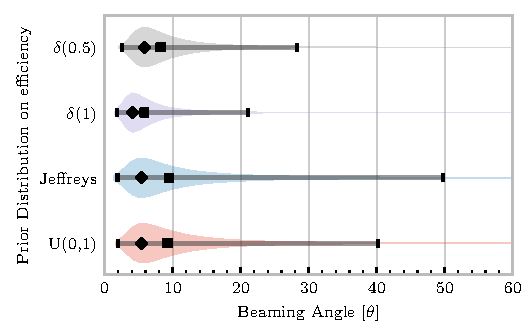
\includegraphics{figures/sgrb/O1_beaming_posteriors_violin.pdf}
  \caption{The posterior probability distribution of the jet
    beaming angle using different priors on the SGRB production
    efficiency in the 2015-2016 observing scenario. \label{fig:o1posterior}}
  \end{figure}

\begin{figure}[b]
  \checkoddpage
  \makebox[\textwidth][\ifoddpage r\else l\fi]{
    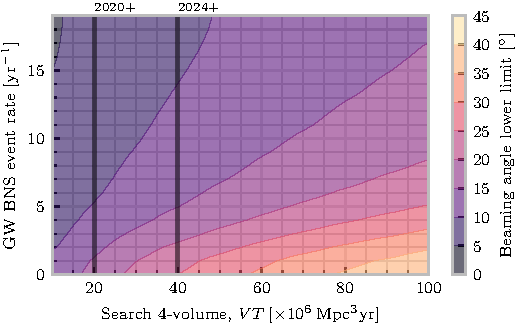
\includegraphics[width=0.9\textwidth]{figures/sgrb/volume_v_nevents_lower.pdf}
    \includegraphics[width=0.9\textwidth]{figures/sgrb/volume_v_nevents.pdf}
  }
   
  \caption{
    The lower [left panel] and upper [right panel] bounds of
    the 95\% credible interval on the beaming angle as a function of
    the rate of observed gravitational wave BNS events, and the
    observed search 4-volume, taking a Jeffreys prior on the
    efficiency of SGRB production from BNS events. The search volumes
    corresponding to anticipated observing scenarios are marked as
    heavy vertical lines on the plot, each assuming observations are
    conducted for one year.
    \label{fig:beaming-jeffreys}
    }
\end{figure}

\begin{figure}[b]
  \checkoddpage
  \makebox[\textwidth][\ifoddpage l\else r\fi]{
    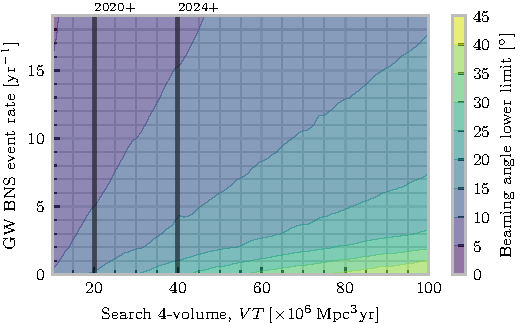
\includegraphics[width=0.9\textwidth]{figures/sgrb/volume_v_nevents_lower_e1.pdf}
    \includegraphics[width=0.9\textwidth]{figures/sgrb/volume_v_nevents_e1.pdf}
  }
   
  \caption{
    The lower [left panel] and upper [right panel] bounds of
    the 95\% credible interval on the beaming angle as a function of
    the rate of observed gravitational wave BNS events, and the
    observed search 4-volume, taking a $\delta(1.0)$ prior on the
    efficiency of SGRB production from BNS events. The search volumes
    corresponding to anticipated observing scenarios are marked as
    heavy vertical lines on the plot, each assuming observations are
    conducted for one year.
    \label{fig:beaming-1}
    }
\end{figure}

Taking the method used to produce \ref{fig:o1posterior} we produced
\ref{fig:beaming-jeffreys} and \ref{beaming-1} which display the upper
and lower bounds on the 95\% credible interval of the beaming angle
posterior at a range of $VT$ values, and a range of BNS rates for a
Jeffreys (comparatively uninformative) and a $\delta(1.0)$ prior.

Our method provides a new means to calculate the beaming angle of
SGRBs without requiring coincident detection of SGRB and BNS events,
and without assuming perfect efficiency in jet production within a
Bayesian framework, and is an example of a Bayesian hierarchical
model, as there are multiple dependent inference steps in the
model. As a result this method is well-suited to be included within a
larger hierarchical analysis framework.


\section{Gaussian Processes for Waveform Modelling}

While the era of observational gravitational wave astrophysics
promises to bring many new insights into previously observable
strong-gravity regimes, it also brings new technological
challenges. One of these concerns the analysis of the observed data,
and our ability to infer the properties of a system which generated a
detected signal. At present, in the case of compact binary coalescence
(CBC) events, this process of \emph{parameter estimation} (PE) is
conducted using matched template filtering, a process which compares
data to precomputed \emph{template} signals. Given a large number of
templates, the match between a signal and each template can be
calculated, with the template which matches the data best representing
the parameters which best describe the observed signal.

Producing template waveforms for CBC events is computationally costly,
requiring numerical relativity (NR) simulations to be carried out,
which may take days or weeks to complete. This high computational cost
limits the number of templates which can be produced, which in turn
limits the precision with which the parameters of the observed system
can be inferred. To get around this problem a number of interpolants
have been produced, including \imrp{} and \seobnr{}, which attempt to
fit deterministic analytical functions to existing NR-produced
waveforms in order to create a function which can be evaluated at any
point withing the parameter space.

These methods have been successful to date, and are used in current
data analysis pipelines for advanced LIGO and advanced Virgo data,
however they are unable to incorporate a measure of the uncertainty of
a prediction at any point in their parameter space. This results in
biased inferences, since the accuracy of the generated template is
unknown.

In an attempt to incorporate this uncertainty there have been attempts
to model the difference between the interpolant and the NR data over
the parameter space\cite{2014PhRvL.113y1101M,2016PhRvD..93f4001M}
using Gaussian Process Regression, allowing a measure of the
uncertainty in the interpolant to be estimated and included in the
inference procedure. We have adapted this idea, but have attempted to
model the entire function (and not just the difference between the
predicted and simulated data) using Gaussian Process Regression.

Gaussian Process Regression (GPR) is a non-parametric Bayesian
regression technique which uses Gaussian Process (GP) priors to
produce plausible fitting functions for supplied data. A GP, when
conditioned on data, provides a posterior probability distribution of
fitting functions; any draw from this distribution is therefore a
plausible interpolant for the data. Analytical forms exist for the
mean and variance of the posterior distribution, allowing a mean
fitting function, and an associated variance to be inferred from the
observed data.

We use a Gaussian Process conditioned off data from around 350
waveforms from the Georgia Tech waveform catalogue\cite{gatechcat} to
produce our interpolation model, which contains around $12\,000$
observations over $11$ parameters, producing an $11$-dimensional
\emph{input} space.

Gaussian Processes are \emph{kernel methods}, and as such they model
data in an inner product space in which distances are relative to
other points within the data, and not to an absolute point. These
methods require that a metric be defined on the data space, which
forms the \emph{covariance function} of the GP.

The covariance function from the HERON model takes the form
\begin{align}
  \label{eq:heron-kernel}
  \Con_0 ( \Con_1 \Mat^{t}_1 + \Con_2 \Mat^{t}_2 ) &\times \Con_3 \SE^{q} 
  \times \Con_4 \SE^{L_x,L_y,L_z} \nonumber \\ 
  &\times \Con_5 \SE^{s_{1,x}, s_{1,y}, s_{1,z}} \nonumber\\ &\times \Con_6 \SE^{s_{2,x}, s_{2,y}, s_{2,z}}
\end{align}
where the superscripts indicate which dimensions of the dataspace are
modelled by each kernel. In the case of the squared exponential
kernels acting on the dimensions of $\vec{L}$, $\vec{s_1}$, and
$\vec{s_2}$, each kernel has three hyperparameters, for the scale
parameter of each dimension, which results in a kernel with eighteen
hyperparameters. The sans serif quantities represent the various
component kernel functions, $\SE$ is the squared-exponential, $\Con$
is a constant kernel, and $\Mat$ represents a Matern-5/2
kernel\footnote{In the interests of brevity the descriptions of these
  functions are omitted from this report, but the interested reader is
  directed towards \cite{rasmussen2006gaussian} and
  \cite{barberBRML2012} for discussion of these functions.}. The total
HERON covariance function is a product of several kernels, allowing
different behaviour of each physical parameter when mapped to the
feature space.

\begin{figure}
  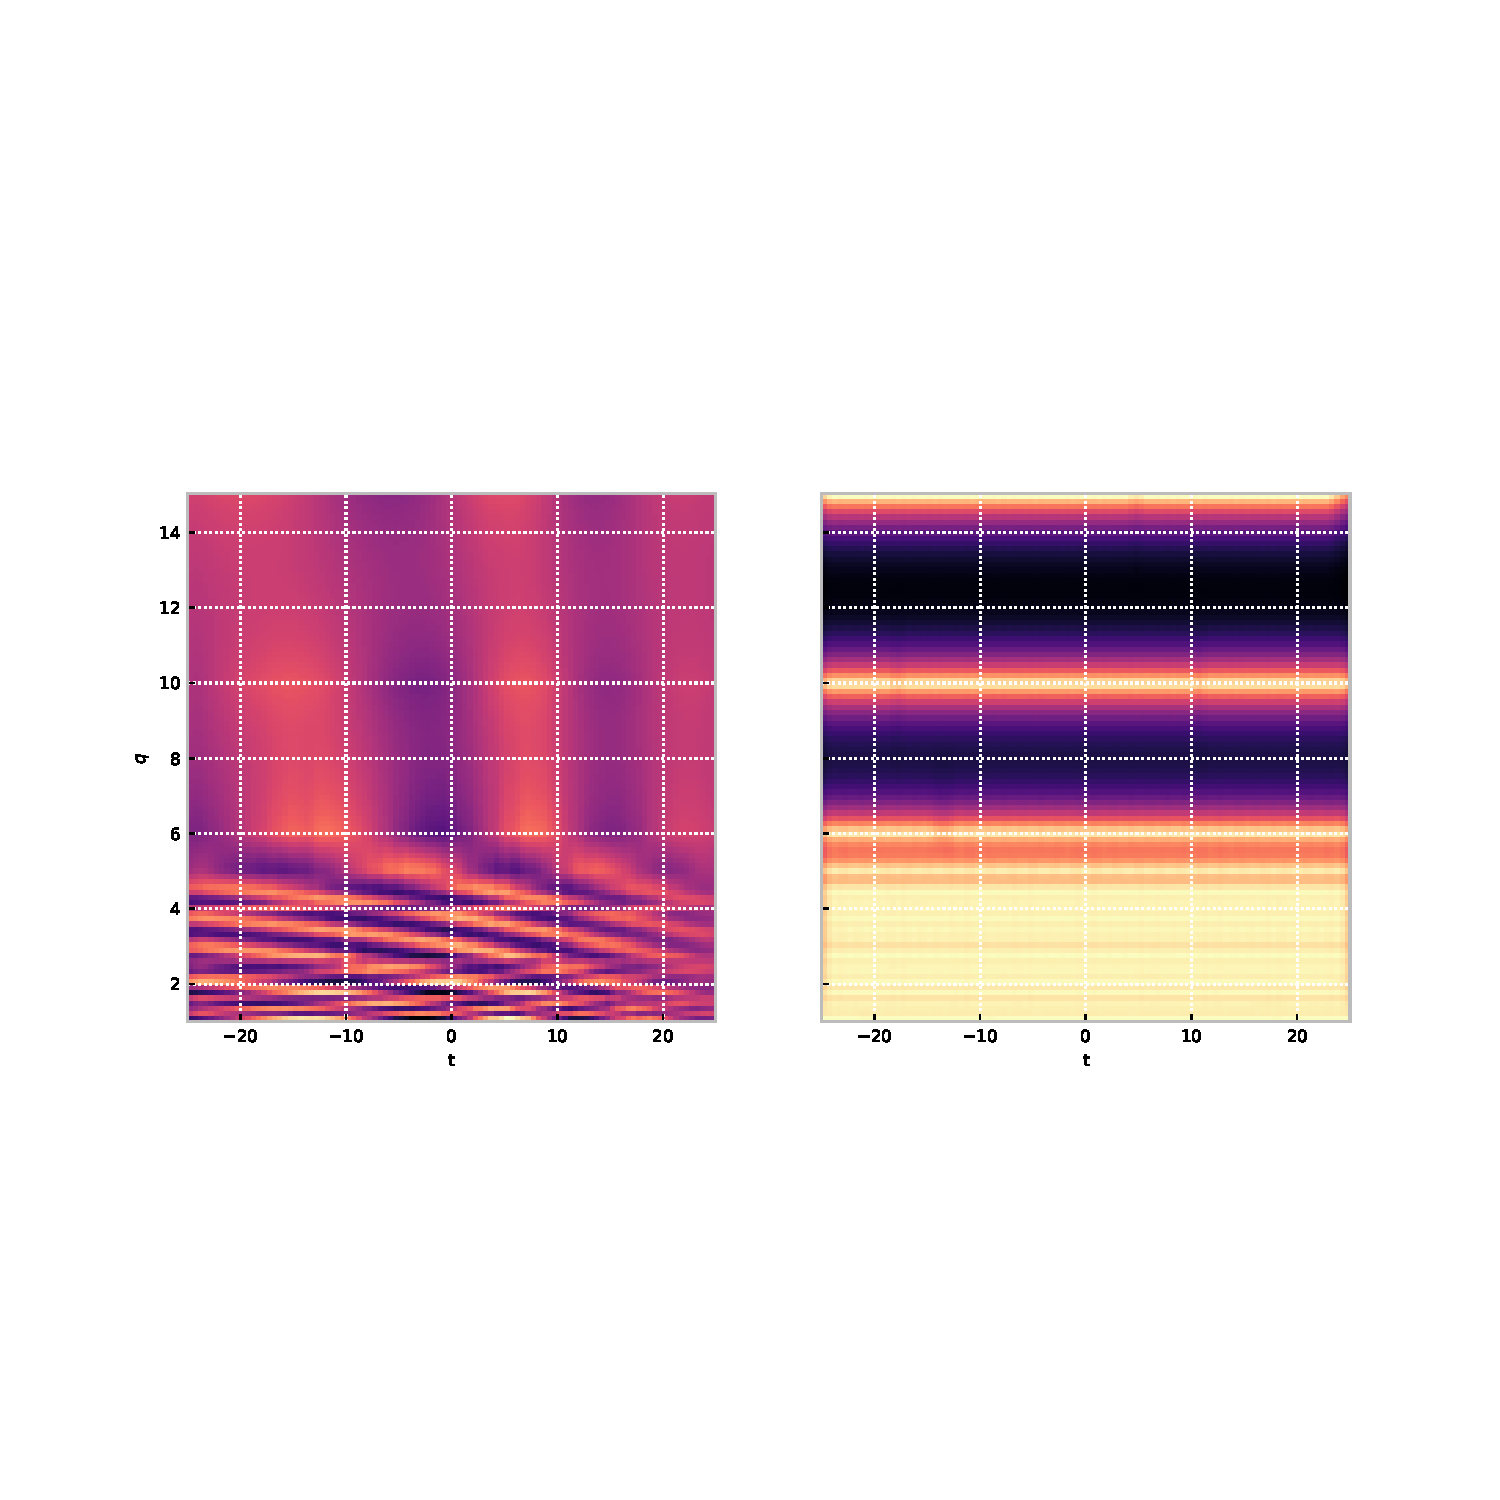
\includegraphics[width=\textwidth, trim={1cm 6cm 2cm 7cm},clip]{figures/heron/monster_qplane.pdf}
  \caption{The output of the full \heron{} model over the $t-q$-
    (time/mass-ratio)-plane for non-spinning waveforms. The panel on
    the left represents the predicted mean function value at each
    point, while the right panel represents the variance of the
    prediction at each point. \label{fig:qtplane}}
\end{figure}

In the case of a surrogate model such as HERON it is important that
the predictions of the model can be tested against data which is known
to be accurate; to accomplish this with our model we set-aside a
number of the training waveforms from the available training
catalogue, and then compare the predictions of the model at the
locations in parameter space at which these waveforms were produced to
the test data itself.

Having a working surrogate model which can produce a measure of the
uncertainty (in the form of the prediction variance) throughout the
model parameter space allows regions which are poorly informed to be
located; such poorly-informed locations are an indication that future
numerical relaitivity simulations should be conducted at those
locations in order to improve our understanding of the waveform
manifold. Gaussian process regression is therefore a promising method
for guiding future waveform placement in a principled and
evidence-based manner. 

\chapter{Thesis Plan}
\chapterprecis{}

\begin{enumerate}
\item Front-matter
  \begin{enumerate}
    \item Acknowledgements
    \item Abstract
  \end{enumerate}
\item Chapter 1: Gravitational waves and their detection
  
  The first detection of gravitational waves in summer 2015 came
  almost one hundred years after the first formualtion of general
  relativity in 1915, and of a wave solution to its field equations
  in 1916. While their detection heralded the beginning of a new field
  of observational astrophysics, this was built on a foundation of
  research and development over the previous century. This chapter
  will contain a brief overview of the technological developments
  which were required to make the detection, the theory of how
  gravitational waves are produced and propogate, and the
  astrophysical sources which are expected and observed to produce
  gravitational waves.
  \begin{enumerate}
  \item Gravitational waves out of general relativity
    
    [ Progress: 0\% ]
    
    This section will be a brief review of the aspects of General
    Relativity which are required to understand gravitational wave
    production and detection; as the bulk of this work does not relate
    to general relativity directly this will be a short summary only,
    and aspects of numerical relativity techniques relevent to the
    generation of waveforms will be reviewed.
    \begin{enumerate}
    \item Brief overview of the generation of GWs
     \item Brief overview of the propogation of GWs
     \item Brief overview of Numerical relativity
    \end{enumerate}

    
 \item An overview of gravitational wave detectors

   [ Progress: ~40\% ]
   
   This section will contain a short historical overview of detector
   technology, and a review of the technological challenges and noise
   sources which modern detectors face, as a motivation for the
   requirement for advanced data analysis techniques, and noise
   modelling. If work on Gaussian process regression for modelling
   Newtonian noise is sufficiently advanced this would call for an
   expanded section on Newtonian noise specifically.

   \begin{enumerate}
   \item A brief history of GW detectors
   \item Noise sources and their mitigation
   \item Current-generation detectors
   \item Future detectors
   \end{enumerate}

   
\item An overview of sources of gravitational waves

  [ Progress: ~40\% ]
  
   This section will contain a review of the various potential sources
   of gravitational waves, with a focus on Compact Binary Coalesence
   (CBC) and burst sources, as these will constitute the subjects of
   analysis in later sections of this work, but there will also be
   sections summarising continuous and stochastic sources, and the
   most up-to-date observational limits which have been obtained by
   the Advanced LIGO and Advanced Virgo detectors for these sources,
   for completeness.
   \begin{enumerate}
   \item Compact binary coalesence
   \item Burst and transient sources
   \item Continuous wave sources
   \item Stochastic sources
   \end{enumerate}

   
 \item GW150914 - The era of gravitational wave astronomy
   
  [ Progress: ~20\% ]
  
   Given the announcement of the first Gravitational Wave detection in
   2016, it is fitting that a review of the literature relating to its
   observation be included here, with some discussion of the
   consquences of that observation. There will also be a brief
   overview of the remainder of the O1 and O2 observations.
   \begin{enumerate}
   \item Brief overview of GW150914
   \item Brief overview of subsequent BBH detections
   \end{enumerate}

   
 \item GW170817 - The dawn of multimessenger gravitational wave astronomy
  
   [ Progress: $0\%$ ]

   Again, with the observation of a gravitational wave event, closely
   followed by a short gamma ray burst, GW170817, the first
   observation of a binary neutron star coalesence in gravitational
   waves, in summer 2017, marked a milestone in modern astrophysics,
   with the confirmation that at least some short gamma ray bursts are
   the result of binary neutron star coalesence. This section will
   contain a brief review of the literature surrounding this
   observation, and the astrophysical inferences which were possible
   as a result of its multimessenger nature, with specific focus on
   the connection between the GW event and the SGRB observation, given
   the contents of chapter 5.
   \begin{enumerate}
   \item Brief overview of GW170817
   \end{enumerate}
  \end{enumerate}

  
\item Chapter 2: Probabilistic reasoning and Bayesian inference
  \begin{enumerate}
\item Probability and Bayes theorem

  [ Progress: $\sim20\%$ ]

   This section will contain an overview of Bayesian reasoning, and
   how it can be applied to data analysis problems, and will contain
   the foundational concepts for the techniques presented later in
   this chapter, including the use of Bayes theorem, and the concept
   of Bayesian updates to a degree of belief interpretation of
   probability.
   \begin{enumerate}
   \item An introduction to Bayesian probabilistic reasoning    
   \item Bayesian methods for data analysis
   \end{enumerate}
   
\item Hierarchical Bayesian problems and structured probability distributions

  [ Progress: $<10\%$ ]
  
   This section will build on the foundations laid in the previous
   section, to summarise and demonstrate how Bayesian inference can be
   used to analyse complex hierarchical problems through the use of
   hierarchical and graphical Bayesian models, and a summary of modern
   techniques for performing such analyses, such as the \texttt{pymc3} Python
   package, and MCMC techniques for numerically computing posterior
   distributions in analytically intractable scenarios.
   \begin{enumerate}
     \item An introduction to hierarchical and graphical Bayesian models
     \item Approximate Bayesian inference in hierarchical models with Monte Carlo techniques
   \end{enumerate}

   
\item Bayesian linear regression
  
   [ Progress: $<10\%$ ]
  
   As a motivation for the use of Gaussian process regression, and as
   an introduction to their derivation, this section will contain a
   brief summary of Bayesian linear regression, a Bayesian regression
   technique which is capable of fitting linear functions to data with
   occamisation built-in to the regression technique. An example of
   the use of this technique will be presented in Appendix B.
   
 \item Gaussian processes
   
   [ Progress: $40\%$ ]
   
   This section will contain a summary of the theory and derivation of
   Gaussian processes, a powerful Bayesian method which can be used
   for non-linear regression, and which is capable of performing fully
   Bayesian function interpolation, including predictive
   uncertainties. This section will also discuss some of the
   computational and implementation challenges of GPR on large data
   sets.  In addition to the foundational theory of GPs and GP
   regression, and details of their implementation, this section will
   introduce the use of Bayesian function optimisation using GPs to
   emulate hard-to-evaluate functions.

   \begin{enumerate}
   \item Bayesian linear regression to Gaussian processes
   \item Gaussian processes - a prior on function spaces
   \item Kernels and covariance functions
   \item Managing computational complexity
   \item Efficient training techniques
   \item Bayesian optimisation using Gaussian process surrogates
  \end{enumerate}
\end{enumerate}
\item Chapter 3: Waveform models for gravitational wave sources

  [ Progress: $<20\%$ (writing), $>95\%$ (programming \& results) ]
  
  This section will contain an overview of the signal morphologies
  which are searched for with advanced gravitational wave
  detectors. First an overview of numerical relativity-derived
  waveforms for CBC gravitational wave sources, which is of great
  relevance to the work of chapter 4 will be given, and similarly an
  overview of NR-derived BNS postmerger waveforms, a prime candidate for
  surrogate-modelling will be included. The available modelled
  supernova waveform morphologies will be summarised, with relation to
  burst searches, and the morphologies which are used in the
  characterisation of the current searches. A section on the models
  which are used to characterise unmodelled searches will be included
  (these are principly sine-gaussian and white-noise burst signals),
  followed by an overview of the three primary search pipelines used
  in Advanced LIGO burst searches (omicron, BayesWave, and Coherent
  Wave Burst), and the details of the method used to characterise
  these pipelines through Mock Data Challenges. A section will
  introduce the production of mock data challenges for burst data
  analysis, and Minke, the toolkit which is used to produce these
  MDCs. Further details of Minke will be included in Appendix
  C. Finally, an overview of waveform approximant models, such as the
  IMRPhenomPv2 family of approximants will be discussed, and previous
  methods used to develop waveforms surrogates will be reviewed in
  preparation for the introduction of a GPR-based approximant in Chapter 4.

  \begin{enumerate}
  \item Modelled waveforms: Binary black holes and binary neutron stars
    \begin{enumerate}
      \item Numerical relativity simulations of BBH
      \item Numerical relativity simulations of BNS post-merger signals
    \end{enumerate}
    
  \item Modelled waveforms: Supernovae
    \begin{enumerate}
    \item Numerical relativity simulations of SNe
    \end{enumerate}
    
  \item Unmodelled waveforms: Analytical models
    \begin{enumerate}
    \item An overview of signal morphologies
    \end{enumerate}
    
  \item overview of burst signal detection
    \begin{enumerate}
    \item Burst search signal detection and analysis
    \item An overview of burst searches in the advanced detector era
    \end{enumerate}
    
  \item Mock data challenges and Minke
  \item Waveform approximants
    \begin{enumerate}
    \item IMRPhenomPv2   
    \item SEOBNR
    \item Spline-based surrogates
    \item Gaussian processes to model waveform uncertainty
    \item Gaussian processes surrogate in a ROM basis
    \end{enumerate}
  \end{enumerate}
\item Chapter 4: Gaussian processes as a surrogate for numerical relativity
  
  [ Progress: $\sim 50\%$ (writing), $>50\%$  (programming \& results) ]

  This
    section will introduce and discuss the HERON Gaussian
    process-based BBH waveform approximant. The first half of this
    section will build on the work presented in Williams, Heng, and
    Gair (in prep), while it is hoped that the later sections (on
    planning future simulations, comparing systematics, and producing
    surrogates for other waveform morphologies) will build upon
    subsequent publications.

    \begin{enumerate}
    
    \item The role of waveforms in GW searches and data analysis
      
   This section will contain a brief overview of matched filtering in
   order to motivate the need for a waveform interpolant, and will
   discuss the probabilistic aspects of the technique to motivate the
   development of a template bank with a measure of interpolation
   uncertainty.   
 \item Building a Bayesian template bank for binary black hole waveforms
   
   This section will cover the details of the construction of the
   HERON GPR model trained off waveforms from the Georgia Institute of
   Technology BBH waveform catalogue, its training, and the choice of
   covariance function used to construct the model. This section will
   also contain details about the training catalogue and testing
   catalogues used to produce the surrogate.
 \item Testing and verifying the model
   
   This section will detail the process of testing the predictions of
   the model against the test set which was held back from the
   original training process in order to validate the predictions of
   the surrogate.
 \item Planning future waveform simulations
   
   The probabilistic nature of the Gaussian process surrogate provides
   a measure of the model's uncertainty across its entire parameter
   space. This section will describe a method for utilising this
   uncertainty to motivate the choice of future parameters for
   numerical relativity simulations in order to best improve the
   surrogate model.
 \item Comparing systematics between template banks
   
   [Possible section]

   With a means of producing a probabilistic model conditioned on
   numerical relativity data, we are afforded a means of comparing the
   difference between two sets of waveforms generated with different
   NR codes, without requiring that the two codes are run at the same
   locations in parameter space. This section would discuss an
   information-theoretic comparison of waveform catalogues using such
   a method.
 \item Gaussian processes for binary neutron star waveforms
   
   Having developed a technique to interpolate BBH waveforms, this
   section will turn to the use of the same technique with an adapted
   covariance structure to the modelling of binary neutron star
   waveforms; understanding the ringdown section of these waveforms
   will be of considerable importance as more BNS detections become
   available.
    \end{enumerate}
\item Chapter 5: Hierarchical Bayesian methods for gravitational wave astronomy

  [ Progress: $>70\%$ (writing) $>95\%$ (programming) ]
  
  This section will cover the use of hierarchical modelling for the
  measurement of astrophysical quantities from gravitational wave and
  electromagnetic observations. The bulk of this section will be based
  around the work presented in Williams et al. (2018)\footnote{In
    press.} relating to the inference of GRB jet angles from
  astrophysical rates. This section will then expand upon the material
  in the paper, to include discussion of inference in situations where
  the GRB rate is modelled as a posterior distribution, and to
  situations where sub-luminous bursts, such as GRB170817A can be
  accounted for within the framework.

  The method used for EM/GW multimessenger observations can be readily
  transferred to scenarios where the are either additional messengers
  (for example high-energy neutrino emission), or where the messengers
  are a mixture of beamed and non-beamed electromagnetic
  emission. This chapter will therefore contain discussion about how
  such a rates-based method can be extended to these regimes within a
  hierarchical modelling framework.

  Finally, this chapter will include discussion of on-going work and
  development of a hierarchical Bayesian pipeline designed for
  coincident detection of multimessenger SGRB events, which will take
  data from both gamma ray observatories and gravitational wave
  observatories to perform inference on the underlying physical
  properties of the SGRB and its progenitor system.

  \begin{enumerate}
  \item Hierarchical inference to infer physical properties from astrophysical rates
  \item Inferring SGRB beaming angles from rate information
  \item Hierarchical modelling for general beamed emission scenarios
  \item A hierarchical model for SGRB astrophysics
  \end{enumerate}
\item Back matter
  \begin{enumerate}
  \item Appendix A: Mathematics for Gaussian process regression

    This appendix will be reserved for derivations and mathematical
    asides which would be disruptive to the flow of the main
    discussion of Gaussian process regression, but which are a useful
    aide to understanding this method. Examples of material which may
    be included here are the algorithm for computing the predictions
    of a Gaussian process, and detailed insights into the linear
    algebra required for this process.
    
  \item Appendix B: The effect of compact objects on pulsar timing arrays

    This appendix will contain discussion of the additional work
    completed on a project started in 2014 on using pulsar timings to
    detect compact objects such as black holes and neutron stars, with
    additional discussion of the effects these objects have on pulsar
    timing arrays.
    
  \item Appendix C: Minke, a toolkit for gravitational wave signal-set creation

    This appendix will contain summary documentation\footnote{Full API
      documentation will be included in a separate publication} of the
    Minke package, along with usage examples.
    
  \item Appendix D: Graphical methods for signal processing

    This appendix will contain an overview of graph-theoretic concepts
    vital to understanding the discussion of hierarchical Bayesian
    modelling in the main body of the thesis.
    
  \item Glossary
  \item Index
  \item References \& bibliography
  \end{enumerate}
\end{enumerate}


\chapter{Future Plan}\chapterprecis{}

In the next ten months I intend to start completing a number of
projects, with the major work being required on the completion and
writing-up of the Gaussian process regression work, and the LSC
collaboration paper on the results of the O2 all-sky burst searches. A
number of smaller projects are also very close to completion, leaving
space for a number of projects to continue previous projects,
especially with regard to gamma ray burst astrophysics and Gaussian
processes. I currently plan to start writing my thesis around October
2018, and aim to have completed most of these projects, or at least
brought them to a mature state by the end of January 2019 in order to
focus on thesis-writing in spring 2019. An approximate overview of
these projects, and their dependent relationships is shown as a Gantt
chart in figure \ref{fig:gantt}.

\section{Near-completion projects}

I currently have two projects which are very close to completion, and
are in the process of being written-up as potential publications; the
first, on the use of pulsar timings to detect EM-dark compact objects
in the local neighbourhood of the Earth (or to place limits on the
nearest such objects) is in a mature state, with work still required
on the manuscript. The second project, on publishing the documentation
for Minke, the MDC-creation tool for GW burst searches is similarly
mature, with the need to refactor existing material for publication in
some form.

\section{Gamma ray burst astrophysics}

Following the publication of \cite{2017arXiv171202585W} as an initial
description of a method to infer jet astrophysics from SGRB and BNS
rates I aim to extend this method to include a more astrophysically
reasonable SGRB rate which takes the distance to the source into
account\footnote{The published version assumes a constant rate
  throughout space}, which would allow the method to take
``subluminous'' SGRB events into account, and would allow inference on
the parameters of more complex models than the ``top-hat'' model
assumed in the published method.

In addition to work on a rates-based method for examining jet physics,
I am collaborating with Fergus Hayes, Connor Isaacs, John Veitch,
Chris Messenger, and Siong Heng on development of a hierarchical
analysis of gravitational wave data to determine astrophysical
parameters, which we hope will eventually be capable of folding-in our
rates-based method. This project is approaching a publishable state,
however I do not anticipating having major involvement in the writing
of this paper.

\section{LSC Collaboration}

I am currently involved with producing the mock data challenge for the
O2 all-sky burst search within the LIGO Scientific Collaboration, and
I am a member of the paper-writing team for the results paper
following this analysis. Under the current schedule this paper is
expected to be finished in late July 2018.

\section{Gaussian process regression projects}

The first strand of the GPR project, the production of a surrogate
model for BBH waveforms, is nearing completion, with a hopeful
timeline of having a publication ready for submission in early summer
2018. Beyond this I hope to complete the second strand of the project,
on a method for the placement of future waveform simulations, by late
summer or early autumn 2018. Additionally, I hope to be able to
build-out the work I have done in collaboration with James Clark at
Georgia Tech on the modelling of BNS post-merger signals in order to
produce a surrogate model for these in a similar manner to the BBH
surrogate.

I also have the possibility of working on GPR as a method for
improving the measurement of Newtonian Noise in gravitational wave
detectors; this project is in very preliminary stages however, and it
is not clear what the probability of this returning substantial
results in the next year is.

\begin{figure}[t]

  \begin{ganttchart}[
%x unit=1cm,
y unit title=.6cm,
y unit chart=.7cm
]{1}{12}
\gantttitle{2018 / 2019 Academic Year}{12} \\
\gantttitlelist{5,...,12}{1} \gantttitlelist{1,...,4}{1} \\
\ganttgroup{Near-completion projects}{1}{3} \\
\ganttbar{Minke documentation}{2}{3} \\
\ganttmilestone{Minke documentation}{3}\\
\ganttlink{elem1}{elem2}

\ganttbar{Pulsar timings}{2}{2}\\
\ganttmilestone{Pulsar timings}{3}\\
\ganttlink{elem3}{elem4}

\ganttgroup{GRB Astrophysics}{1}{10}\\

\ganttbar{Subluminous GRB Beaming}{4}{7}\\
\ganttmilestone{GRB Beaming II}{7}\\
\ganttlink{elem6}{elem7}

\ganttbar{Hierarchical GRB Model}{1}{3}\\
\ganttmilestone{GRB Astrophysics I}{4}\\
\ganttlink{elem8}{elem9}


\ganttgroup{LSC Collaboration Work}{1}{5}\\
\ganttbar{O2 All-sky Analysis}{1}{3}\\
\ganttmilestone{O2 All-sky Analysis}{5}\\
\ganttlink{elem11}{elem12}

\ganttgroup{GPR Projects}{1}{8}\\

\ganttbar{GPR Predictive Surrogate}{1}{1} \\
\ganttbar{GPR Placement Criteria}{3}{4} \ganttnewline
\ganttmilestone{GPR Surrogate I}{2}\\
\ganttlink{elem14}{elem15}
\ganttlink{elem14}{elem16}
\ganttmilestone{GPR Surrogate II}{5} \\
\ganttlink{elem15}{elem17}
\ganttbar{GPR Newtonian Noise}{4}{5}\\
\ganttbar{GPR BNS Postmerger}{3}{5}\\

\ganttgroup[
group/.append style={fill=muted-blue}
]{Thesis}{6}{11}\\
\end{ganttchart}

\caption{A Gantt Chart for the next ten months' worth of work and
  publications. Diamonds represent publications, while un-filled boxes
  represent distinct sub-projects. Filled bars indicate project groupings.\label{fig:gantt}}
  
\end{figure}

\chapterstyle{minimalist}
\newgeometry{left=1.5in,right=1.5in, top=6cm}
\bibliographystyle{unsrt85}
%\begin{multicols*}{2}% two columns
  \linespread{.8}
  \bibliography{bibliography/introduction,bibliography/relativity,bibliography/detectors,bibliography/gw150914,bibliography/sources,bibliography/analysis,bibliography/gaussian}
%  \end{multicols*}
%\restoregeometry
\end{document}
